%--------------------------------------------------------------------------------------------------
\chapter{Aufbau des Konzepts}\label{cha:AufbauDesKonzepts}
In diesem Kapitel wird der Aufbau des Konzepts erklärt. Daher gibt es zuerst einen Einblick in den Prozess von der physischen Produktionsanlage bis hin zu ihrem virtuellen Klon. Daraufhin wird diese Arbeit in das Gesamtkonzept der Mensch-Maschine Interaktion eingeordnet. Anschließend werden Anforderungen definiert und der grobe Aufbau des Modells erläutert, bevor in einem Ausblick der FMI Standard und dessen Potenziale thematisiert werden.

%Anschließend wird ein Modell mit Hilfe des Functional-Mockup Interfaces aufgestellt. %Schließlich gibt es einen Einblick in die Potenziale des Functional-Mockup Interfaces.

%--------------------------------------------------------------------------------------------------
\section{Digitalisierung der Produktion}\label{sec:PhysischZumKlon}
Die Produktionsabläufe einer Fabrik in einer virtuellen Welt abzubilden, erfordert, nach Rücksprache mit meinem Betreuer, insgesamt sieben Schritte die befolgt werden müssen:
\begin{enumerate}
	\item \textbf{Scannen der Fabrik} \\
	Im ersten Schritt werden die Produktionsräume inklusive der Produktionsanlagen gescannt. Das Ergebnis dieses Scans ist eine Punktwolke.
	\item \textbf{Umwandlung des Scans} \\
	Der Scan muss von einer Punktewolke in CAD Modelle umgewandelt werden. Da die CAD Modelle zu groß und daher unpraktikabel für die Entwicklungsumgebung Unity sind, werden diese in das OBJ Format umgewandelt. Die Modelle sind für den späteren Aufbau des virtuellen Klons der echten Produktionsanlage notwendig.
	\item \textbf{Abbildung: Produktionsanlage $\rightarrow$ Modell} \\
	Es wird ein physisches Modell zur Darstellung einiger wichtiger Herausforderungen der echten Produktionsanlage gebaut. Dies könnte beispielsweise die Form einer Produktionsstraße mit mehreren Stationen besitzen.
	\item \textbf{Virtueller Aufbau} \\
	Das physische Modell der echten Produktionsanlage aus Schritt drei wird in der virtuellen Welt abgebildet (virtueller Klon) und mit dem Menschmodell begehbar gemacht. Dieser Schritt erlaubt die virtuelle Planung einer Produktionsanlage.
	\item \textbf{Konnektivität und Kommunikation} \\
	Die Produktionsanlagen des physischen Modells werden mit der Cloud vernetzt um eine bidirektionale Kommunikation zwischen dem physischem Modell und dem virtuellen Klon zu ermöglichen.
	\item \textbf{Interaktion} \\
	Die Interaktion mit zwischen dem Bediener und den Produktionsanlagen in der virtuellen Welt wird implementiert. Es müssen unter Umständen anwendungsspezifische Benutzeroberflächen implementiert werden.
	\item \textbf{Skalierung} \\
	Skalierung der Vorgehensweise durch Anwendung von Schritt vier bis sechs auf die echte Produktionsanlage.
\end{enumerate}
Das Ergebnis dieser sieben Schritte ist ein virtueller Klon der echten Produktionsanlage. Dieser virtuelle Klon kann für viele verschiedene Zwecke eingesetzt werden, dazu gehören beispielsweise die Produktionsplanung oder das Fernsteuern von Produktionsanlagen. Das Ergebnis dieser Arbeit kommt bei Schritt vier und sechs zum Einsatz.

%--------------------------------------------------------------------------------------------------
\section{Mensch-Maschine Interaktion}\label{sec:MMInteraktion}
\begin{figure}[h]
	\centering
	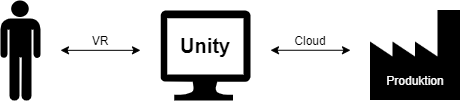
\includegraphics[width=0.7\linewidth]{Bilder/A19_MMI}
	\caption{Die Mensch-Maschine Interaktion im Kontext dieser Arbeit, eigene Abbildung}
	\label{fig:MMI}
\end{figure}
\noindent Durch die Abbildung der echten Produktionsanlage in der virtuellen Welt findet die Mensch-Maschine-Interaktion in zwei Schritten statt. Im ersten Schritt interagiert der Mensch mit der Software (dem Computer) über VR-Hardware. Dieser Computer interagiert dann im zweiten Schritt (z.B. über eine Cloud) mit der echten Produktionsanlage. Die Kommunikation findet in beiden Schritten bidirektional statt.
\newline
Diese Arbeit befasst sich mit dem ersten Schritt der oben erklärten Mensch-Maschine Interaktion. Für den weiteren Verlauf dieser Arbeit wird angenommen, dass es bereits eine geeignete Infrastruktur für die Kommunikation zwischen dem Computer und der Produktionsanlagen über eine Cloud gibt.

%--------------------------------------------------------------------------------------------------
\section{Interaktivität mit einem Menschmodell}\label{sec:ModellAufbau}
Basierend auf den im folgenden definierten Anforderungen sollen das Menschmodell und die Interaktionsschnittstelle aufgebaut werden.

\subsection{Die Anforderungen an das Modell}\label{sec:AnforderungenKonzept}
Das Modell besteht aus zwei Teilen, daher haben beide Teile Ihre eigenen Anforderungen. Diese werden im Folgenden erläutert. Das Ziel ist es ein Menschmodell zu schaffen, welches eine intuitive Interaktion mit der Umgebung ermöglicht.

\subsubsection{Menschmodell}\label{sec:AnforderungenMensch}
\begin{enumerate}
	\item \textbf{Genauigkeit} \\
	Die Genauigkeit der Abbildung der Tracking-Daten auf das virtuelle menschliche Abbild ist von zentraler Bedeutung. Vor allem in einem Szenario, bei dem sich mehrere virtuelle menschliche Abbildungen in einem virtuellen Klon einer Produktionsanlage aufhalten, ist die möglichst genaue Abbildung unabdingbar, um beispielsweise auf andere Bediener in der virtuellen Welt Rücksicht nehmen zu können.
	\item \textbf{Echtzeit} \\
	Sowohl das Tracking des Bedieners, als auch die Abbildung der Tracking-Daten auf das virtuelle menschliche Abbild, sind echtzeitkritische Anwendungen. Die Verzögerungen müssen möglichst gering sein um, eine gute Nutzbarkeit zu ermöglichen.
	\item \textbf{Interoperabilität} \\
	Das Menschmodell muss umgebungsunabhängig implementiert werden. Dies bedeutet, dass das Menschmodell in beliebigen Umgebungen (Fabriken, Produktionshallen, etc.) eingesetzt werden kann.
	\item \textbf{Modularität} \\
	Sowohl einzelne Komponenten, als auch das ganze Menschmodell an sich unterliegen der Anforderung der Modularität, um in Zukunft Verbesserungen oder Erweiterungen am Modell durchführen zu können.
\end{enumerate}

\subsubsection{Interaktion}\label{sec:AnforderungenInteraktion}
\begin{enumerate}
	\item \textbf{Bidirektionalität} \\
	Der Informationsaustausch muss bidirektional stattfinden. Das bedeutet, dass der Bediener über geeignete, leicht zu verstehende, optisch ansprechende und vor allem einheitliche Benutzeroberflächen mit der Umgebung interagieren kann. Einerseits ermöglichen diese Benutzeroberflächen dem Bediener das Interagieren mit Produktionsanlagen, andererseits werden auf diesen Benutzeroberflächen für den Bediener relevante Informationen über die Produktionsanlagen in geeigneter Form dargestellt.
	\item \textbf{Genauigkeit} \\
	Auch bei der Interaktion spielt die Genauigkeit eine wichtige Rolle. Der Bediener sollte intuitiv, mit relativ geringen Lernaufwand, schnell und vor allem präzise mit der Umgebung interagieren können.
	\item \textbf{Echtzeit} \\
	Die Interaktion muss mit einer möglichst geringen Verzögerung stattfinden, um dem Nutzer schnelle Reaktionen und spontane Anpassungen oder Verbesserungen zu ermöglichen.
	\item \textbf{Interoperabilität} \\
	Die Interaktion muss über eine einheitliche Schnittstelle stattfinden, um Interoperabilität zu gewährleisten, sodass sich die Funktionalität auf beliebige Maschinen und Produktionsanlagen übertragen lässt.
	\item \textbf{Modularität} \\
	Durch das Gewährleisten der Modularität wird sichergestellt, dass die Interaktion in Zukunft auch auf neue VR-Hardware übertragen werden kann, ohne das die gesamte Software neu geschrieben werden muss.
\end{enumerate}
Durch das Einhalten dieser Herausforderungen ergibt sich ein Menschmodell, welches in Echtzeit die Bewegungen des Bedieners auf das virtuelle menschliche Abbild projiziert. Des Weiteren ermöglicht das Modell dem Bediener in der virtuellen Welt mit dem virtuellen Klon der Produktionsanlage zu interagieren. Da von Anfang an ein Fokus auf Interoperabilität und Modularität gelegt wird, ist das ganze Modell erweiterbar und an verschiedene Hardware und unterschiedliche Einsatzzwecke anpassbar.
\newpage

\subsection{Der Aufbau des Modells}\label{sec:AufbauModell}
In Abbildung \ref{fig:CodeDarstellung} ist ein stark vereinfachter Überblick über den Aufbau des Codes vom Modell dargestellt. Die blauen Pfeile kennzeichnen den Datenfluss in das Projekt und die grünen Pfeile den Datenfluss aus dem Projekt heraus. Der Bediener nutzt die VR Hardware, welche über das Programm VIVE Wireless mit der VR-Schnittstelle für Computer (SteamVR) verbunden ist. In dem Projekt ist zusätzlich das SteamVR Plugin für die Entwicklungsumgebung Unity installiert, welches die Schnittstelle zwischen dem Projekt und der VR-Hardware vollendet. Zur Verfügung gestellt wird das Modell von dem Plugin „Final IK“ (IK = Inverse Kinematics), welches gleichzeitig die Kalibrierung, die Berechnung der inversen Kinematik und die Abbildung der Bewegungsdaten auf das Modell übernimmt. Die wichtigsten Skripte sind die Skripte CalibrationController und TrackerAssignment. Das Skript CalibrationController ruft zunächst die Methode für die Zuweisung der Tracker in dem Skript TrackerAssignment auf, bevor der Kalibrierungsprozess gestartet wird. Der Kalibrierungsprozess wird standardmäßig mit Hilfe der Positionen der Hände und des Kopfes ausgeführt. Optional können auch die Tracker an den Füßen und dem Steißbein berücksichtigt werden. Durch das Skript TrackerAssignment werden nur die aktiven Tracker den entsprechenden Körperteilen (Füße, Knie, Steißbein, Hände, Ellenbogen, Kopf) zugewiesen. Die entsprechenden Körperteile des Modells enthalten alle das Skript SteamVR Tracked Object, über welches sie die Bewegungsdaten des Bedieners erhalten. Das Ergebnis des Projekts ist das virtuelle Abbild der menschlichen Bewegungen, welches über die zuvor genannten Schnittstellen zurück bis an die VR Hardware geht. Es ist anzumerken, dass das Menschenmodell noch über weitere Funktionalitäten, wie z.B. die Interaktion mit der Umgebung verfügt. Ein genauerer Einblick in den Aufbau des Projekts folgt in Kapitel \ref{cha:Umsetzung}.
\begin{figure}[h]
	\centering
	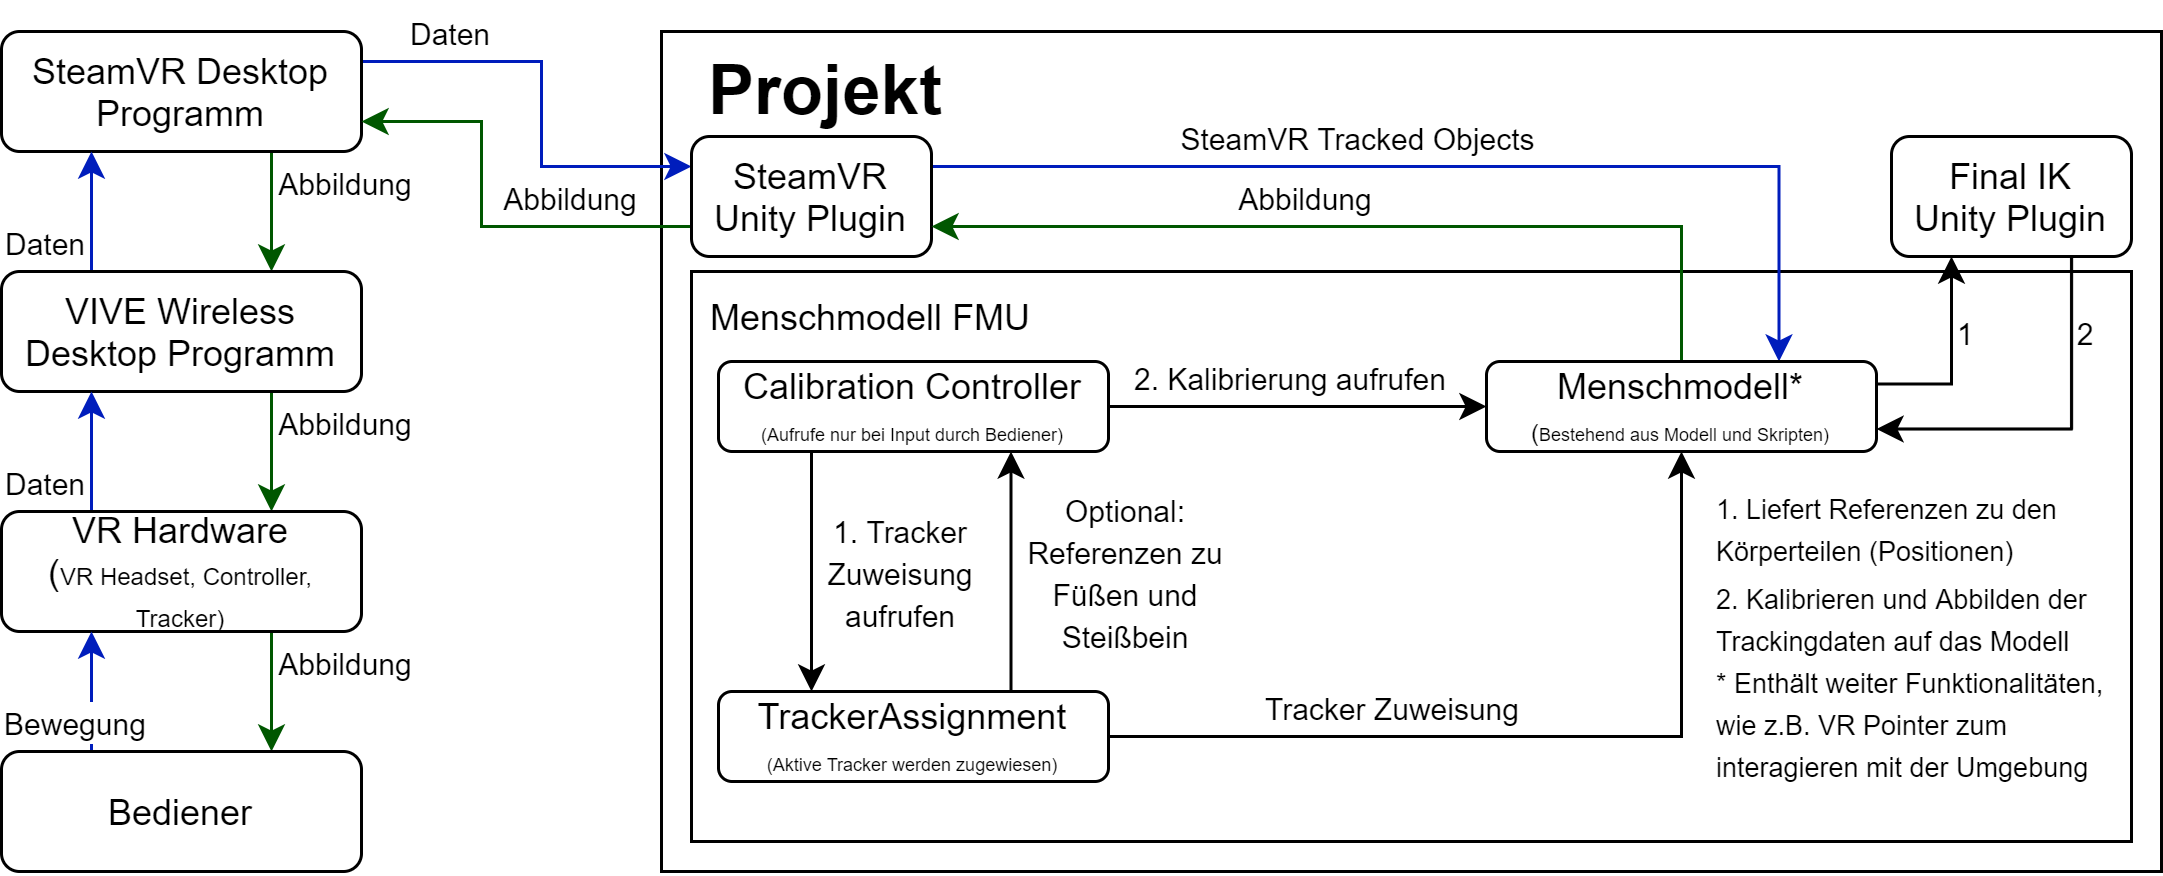
\includegraphics[width=0.9\linewidth]{Bilder/A25_CodeDarstellung}
	\caption{Die grobe Darstellung vom Aufbau des Codes, eigene Abbildung}
	\label{fig:CodeDarstellung}
\end{figure}

\subsection{Ausblick und Erweiterungsmöglichkeit mit Hilfe des FMI Standards}\label{sec:AusblickFMI}
Mit Hilfe des im folgenden Vorgestellten FMI Standards, könnte das in Kapitel \ref{sec:AufbauModell} erläuterte Menschmodell inklusive der Interaktionsschnittstelle erweitert und für den Einsatz in der Industrie vorbereitet werden. Dabei ist anzumerken, dass dieser Ansatz eine noch nicht geprüfte Idee darstellt und daher nur konzeptionell vorgestellt wird.
\newpage

\subsubsection{Das Functional-Mockup Interface}\label{sec:DasFMU}
Das Functional-Mockup Interface (FMI) ist ein ursprünglich von der Daimler AG entwickelter unabhängiger Standard. Zum Einsatz kommt das Functional-Mockup Interface beispielsweise beim Modellaustausch von dynamischen Modellen oder der Co-Simulation zwischen Zulieferern und den OEMs (Original Equipment Manufacturer) \cite[S.1]{24}.
Anfang 2010 wurde die erste Version (Version 1.0) des FMI Standards veröffentlicht, welche zunächst nur den Modellaustausch unterstützte. Einige Monate später folgte dann die Unterstützung für Co-Simulation. Mittlerweile gab weitere Nachfolger Versionen. Die aktuellste Version (Version 2.0.1) wurde im Oktober 2019 veröffentlicht, unterscheidet sich aber von der Vorgängerversion (Version 2.0) aus dem Jahr 2014 nur durch einige Bugfixes \cite[S.2]{25}.
Da es neben den anwendungsspezifischen Standards (z.B. Matlab/Simulink: S-Functions) zunächst keinen unabhängigen Standard für den Austausch von Modellen oder die Co-Simulation gab \cite[S.1]{24}, liegt der größte Vorteil des FMI-Standards in seiner Unabhängigkeit.
\newline
Wie bereits erwähnt gibt es für den FMI Standard zwei übergeordnete Anwendungsszenarien:
\begin{enumerate}
	\item \textbf{„Modellaustausch"} \cite[S.4]{25} \\
	Der FMI Standard ermöglicht Modellierungsumgebungen ein dynamisches System Modell in C-Code zu repräsentieren, sodass dieses Modell auch in anderen Modellierungsumgebungen genutzt werden kann. Ermöglicht wird dies durch die Darstellung der Modelle mit Hilfe von mathematischen Gleichungen (z.B. Algebraische Gleichungen oder Differentialgleichungen), welche auch Events über beispielsweise Zeit- oder Zustandsänderungen enthalten können. Es werden große Modelle und sowohl die lokale als auch die globale Simulation (über das Internet) unterstützt \cite[S.4]{25}.
	\item \textbf{„Co-Simulation"} \cite[S.4]{25} \\
	Des Weiteren ermöglicht der FMI Standard das Verbinden von mehreren Subsystem, welche über vordefinierte Kommunikationsschnittstellen kommunizieren und somit eine Co-Simulationsumgebung schaffen. Dabei wird der Datenaustausch und die Synchronisation zwischen den einzelnen Subsystemen durch einen sogenannten Master Algorithmus gesteuert. Bei den Master Algorithmen ist zu beachten, dass diese nicht zum eigentlichen FMI Standard gehören \cite[S.4]{25}. Daher sind die Master Algorithmen nicht standardisiert und können unterschiedliche zusätzliche Funktionalitäten wie z.B. den Austausch von Variablen unterstützen \cite[S.1]{24}.
\end{enumerate}
Die grundlegenden Komponenten die beim Einsatz des FMI Standards immer zum Einsatz kommen sind das „FMI Application Programming Interface (C)“ und das „FMI Description Schema (XML)“. Ersteres enthält dabei alle benötigten Gleichungen des Models. Dabei kommt die Programmiersprache C zum Einsatz, da sie portabel ist und auch für den Einsatz in eingebetteten System geeignet ist. In der XML-Datei (vgl. Abbildung \ref{fig:FMIOverview}) hingegen werden alle Variablen gespeichert. Die Simulationstools können selber entscheiden, wie sie mit diesen Daten umgehen und wie sie die Daten für den Bediener darstellen möchten. Mit Hilfe der XML-Datei können die Daten, ohne Einbußen bei der Performance, in der gewünschten Programmiersprache (wie z.B. Java oder C\#) verwaltet werden.
\cite[S.8]{25}.
\newpage
\begin{figure}[h]
	\centering
	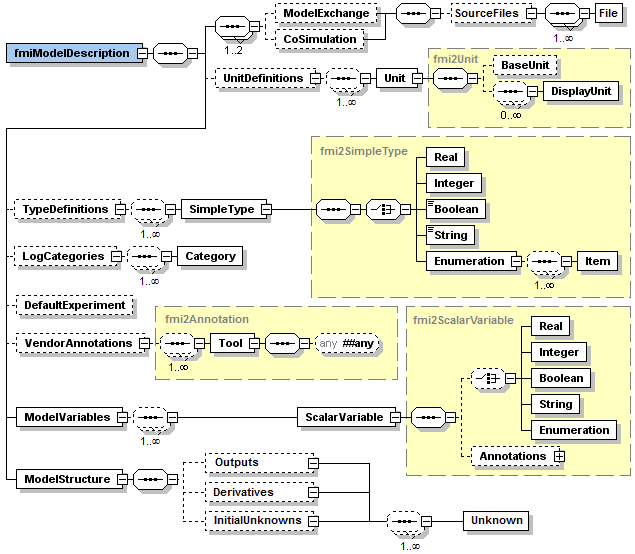
\includegraphics[width=0.7\linewidth]{Bilder/A20_FMIOverview}
	\caption{Der Aufbau der FMI Variablenbeschreibung \cite[S.30]{25}}
	\label{fig:FMIOverview}
\end{figure}
\noindent Da das FMI nur ein Interface ist, wird eine Instanz des Interfaces FMU (Functional-Mockup Unit) genannt. Das FMI Interface soll den Einsatz von FMUs in beliebigen Simulationsumgebungen einfach gestalten. Die Simulationsumgebungen können über Funktionen Instanzen einer beliebigen FMI in Form einer FMU generieren. Es ist zusätzlich anzumerken, dass eine FMU beliebig oft und sogar als Teil von anderen Modellen generiert werden kann \cite[S.8]{25}. Eine FMU wird in einer ZIP-Datei mit der Endung „.fmu“ bereitgestellt und kann neben den bereits angesprochenen Komponenten (C-Code und XML-Datei) zusätzliche Anwendungsspezifische Daten wie Icons oder Dokumentationen enthalten \cite[S.4+9]{25} In Abbildung \ref{fig:FMIBlock} ist eine Instanz einer FMU illustriert. Eine FMU enthält neben den Eingabeparametern (Rot) und den Ausgabeparametern (Blau) noch interne Werte. Zu den internen Werten gehört die Zeit t, interne Parameter p und nach außen sichtbare Variablen v \cite[S.8]{25}.
\begin{figure}[h]
	\centering
	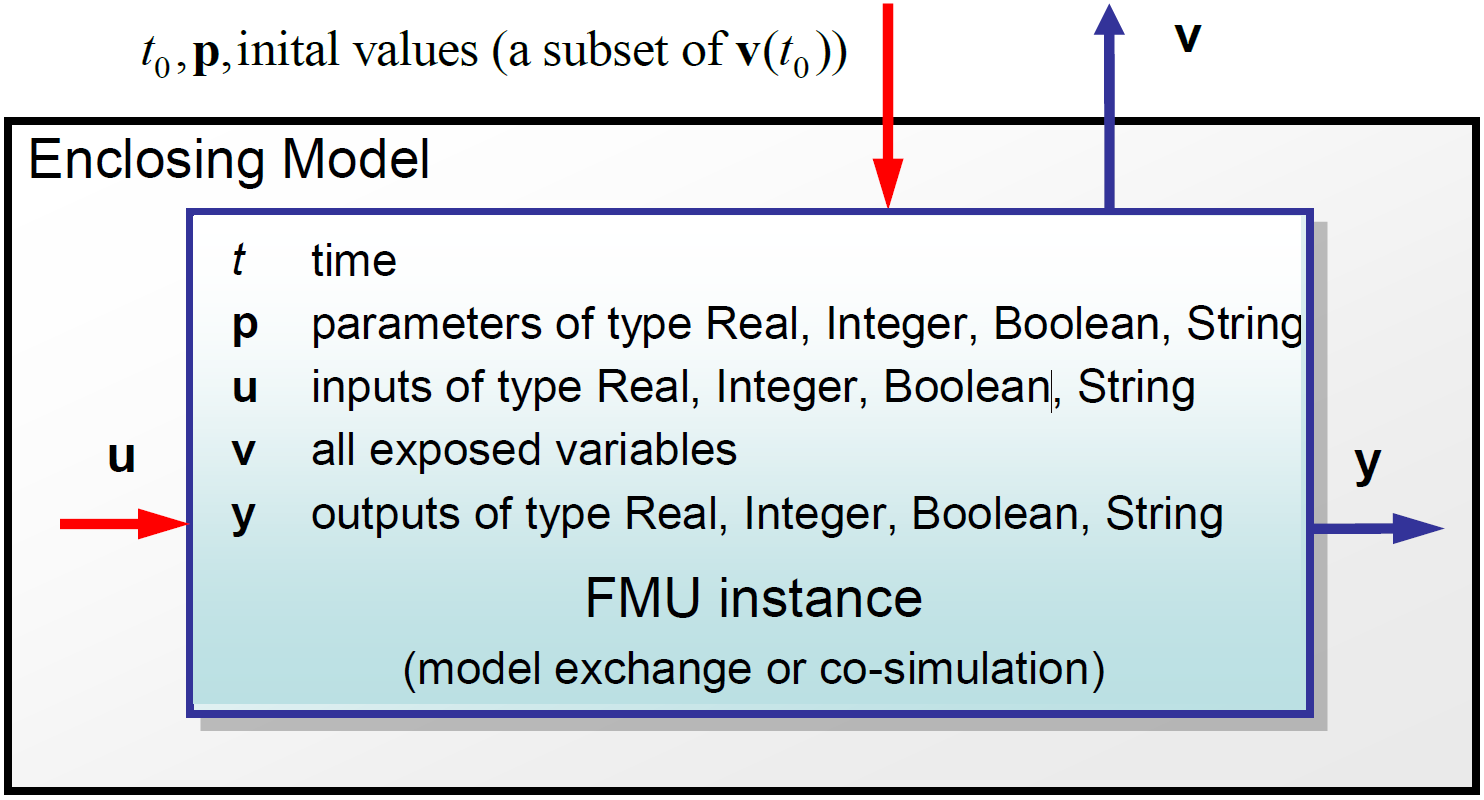
\includegraphics[width=0.5\linewidth]{Bilder/A21_FMIBlock}
	\caption{Die Darstellung einer FMU Instanz \cite[S.9]{25}}
	\label{fig:FMIBlock}
\end{figure}
\newline
In Abbildung \ref{fig:FMUEinordnung} ist noch einmal dargestellt, wie das Zusammenspiel zwischen der Simulationsumgebung, der FMU und dem FMI aussieht. Die Simulationsumgebung liest die Variablendefinition (XML) der FMU, welche dem FMI Standard entspricht. Dies ermöglicht der Simulationsumgebung eine oder mehrere Instanzen der FMU zu generieren. Aufgrund dieser Struktur kann jede Simulationsumgebung eine eigene Benutzeroberfläche einsetzen und selber entscheiden, wie die Daten repräsentiert werden \cite[S.7]{26}.
\begin{figure}[h]
	\centering
	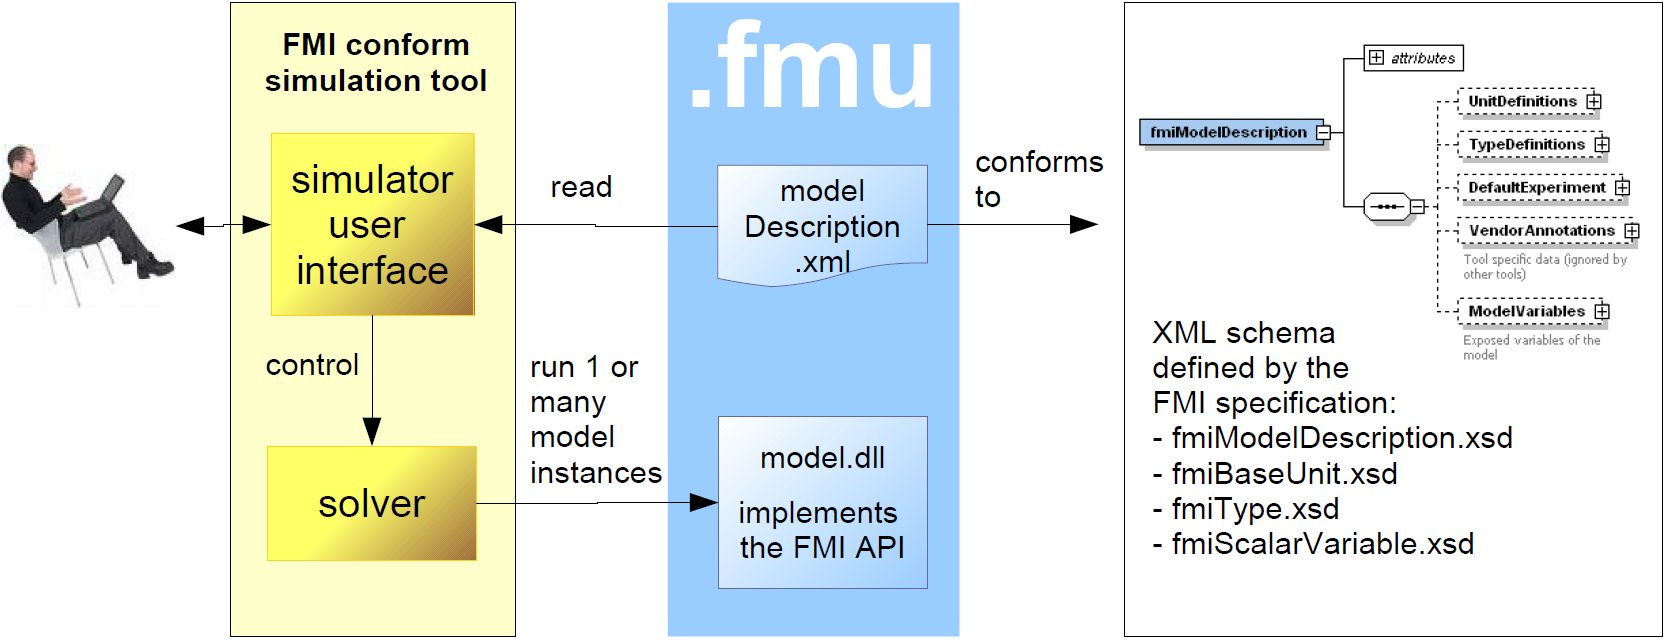
\includegraphics[width=1\linewidth]{Bilder/A22_User-FMU-FMI}
	\caption{Die Funktionsweise der FMU in der Simulationsumgebung \cite[S.7]{26}}
	\label{fig:FMUEinordnung}
\end{figure}

\subsubsection{Der Aufbau des Modells nach dem FMI Standard}\label{sec:ModelAufbau}
Unter Berücksichtigung der in Kapitel \ref{sec:AnforderungenKonzept} erläuterten Anforderungen, soll nach dem Vorbild des in diesem Kapitel eingeführten FMI Standards ein theoretisches Konzept geschaffen werden, welches beschreibt, wie ein Menschenmodell, mit der Möglichkeit mit der Umgebung zu interagieren, nach dem FMI Standard aufgebaut sein könnte. Im Folgenden wird lediglich die Variablendefinition im XML-Format vorgestellt, da das eigentliche Modell (C-Code) eine ähnliche Struktur, wie sie in Abbildung \ref{fig:CodeDarstellung} dargestellt ist, besitzen würde.

\subsubsection{Die Variablendefinition (XML)}\label{sec:Variablendefinition}
\noindent Wie in Abbildung \ref{fig:FMIOverview} dargestellt, besteht die XML-Datei aus mehreren Komponenten. Nicht alle Komponenten sind für jeden Einsatzzweck relevant, daher werden im Folgenden die relevanten Komponenten genauer erläutert.
Es ist zusätzlich anzumerken, dass sowohl wie die XML-Datei an sich, als auch einige der in Abbildung \ref{fig:FMIOverview} dargestellten Elemente zusätzlich über eigene Attribute verfügen. Dies wurde in Abbildung \ref{fig:FMIOverview} aus Platz gründen ausgelassen.
\paragraph{Attributes}\label{sec:AttributeFMU}
\noindent Neben den in Abbildung \ref{fig:FMIOverview} dargestellten Elementen enthält die XML-Datei, wie bereits erwähnt, noch das Element „Attributes“. Es gibt insgesamt 12 mögliche Attribute, jedoch sind nur vier zwingend notwendig \cite[S.33]{25}.
\begin{enumerate}
	\item \textbf{„fmiVersion"} \cite[S.33]{25} \\
	Dieses Attribut gibt an, welche Version des FMI Standards bei der Generierung der XML-Datei
	eingesetz wurde \cite[S.33]{25}.
	\item \textbf{„modelName"} \cite[S.33]{25} \\
	Durch dieses Attribut wird dem Modell ein Name zugewiesen \cite[S.33]{25}.
	\item \textbf{„guid"} \cite[S.33]{25} \\
	Durch das Attribut „guid“ (Globally Unique Identifier) wird sichergestellt, dass die XML-Datei Kompatibel mit den C-Funktionen der FMU ist. Dafür wird in der Regel eine Art Fingerabdruck generiert und in den C-Funktionen hinterlegt \cite[S.33]{25}.
	\item \textbf{„variableNamingConvention"} \cite[S.33]{25} \\
	Dieses Attribut bestimmt, ob die Namen der Variablen einer bestimmten Konvention 
	unterliegen. Standardmäßig wird hier der Token „flat“ verwendet, wenn alle Variablen
	in einer Liste von Strings vorliegen \cite[S.33]{25}.
	\item \textbf{„description" (optional)} \cite[S.33]{25} \\
	In diesem Attribut kann auf Wunsch eine Beschreibung der FMU hinterlegt werden \cite[S.33]{25}.
	\item \textbf{„author" (optional)} \cite[S.33]{25} \\
	Dieses Attribut ermöglicht es Angaben über die Entwickler zu machen \cite[S.33]{25}.
	\item \textbf{„version" (optional)} \cite[S.33]{25} \\
	Mit Hilfe der optional hinterlegten Versionsnummer (z.B. Version 1.0), kann durch dieses Attribut ein besserer Überblick über die verschiedenen Versionen einer FMU ermöglicht werden. \cite[S.33]{25}.
	\item \textbf{„copyright" (optinal)} \cite[S.33]{25} \\
	In diesem Attribut können Informationen über das Copyright hinterlegt werden \cite[S.33]{25}.
	\item \textbf{„license" (optional)} \cite[S.33]{25} \\
	Es besteht die Möglichkeit, durch dieses Attribut Angaben über die Lizenz für die Verwendung
	der FMU zu machen \cite[S.33]{25}.
	\item \textbf{„generationTool" (optional)} \cite[S.33]{25} \\
	In diesem Attribut kann der Name des Tools mit dem die XML-Datei generiert wurde
	hinterlegt werden \cite[S.33]{25}.
	\item \textbf{„generationDateAndTime" (optional)} \cite[S.33]{25} \\
	Dieses Attribut ermöglicht es das Datum und die genaue Uhrzeit der Generierung der XML-
	Datei zu hinterlegen. Dabei wird das Format „YYYY-MM-DDThh:mm:ssZ“ verwendet. Das
	„T“ soll lediglich das Datum von der Uhrzeit trennen und das „Z“ steht für die Zeitzone
	(Greenwich Meantime) \cite[S.33]{25}.
	\item \textbf{„numberOfEventIndicators" (optional)} \cite[S.33]{25} \\
	Falls die FMU für Co-Simulation verwendet wird, wird dieses Attribut ausgelassen. Ansonsten
	wird hier die Anzahl der Indikatoren für Events beim Einsatz der FMU für Modellaustausch
	hinterlegt \cite[S.33]{25}.
\end{enumerate}
\noindent Abbildung \ref{fig:FMUAttribute} illustriert, wie die Attribute für die FMU aussehen könnten.
\begin{figure}[h]
	\centering
	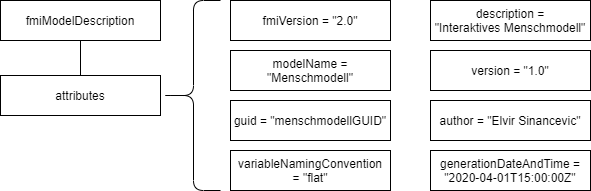
\includegraphics[width=0.9\linewidth]{Bilder/A24_FMUAttributBeispiel}
	\caption{Die beispielhafte Darstellung der FMI Attribute, eigene Abbildung}
	\label{fig:FMUAttribute}
\end{figure}
\paragraph{ModelExchange / Co-Simulation}\label{sec:ModellExchangeCoSimulation}
\noindent Dieses Element gibt an, ob die FMU für Modellaustausch und/oder Co-Simulation ausgelegt ist.
Falls das Element „ModelExchange“ vorhanden ist, enthält die FMU entweder selbst das eigentliche Modell oder die Kommunikationsschnittstelle zu einem Tool, welches das Modell enthält. Die Simulationsumgebung kümmert sich dann um die Simulation.
Falls jedoch das Element „CoSimulation“ vorhanden ist, enthält die FMU selbst das Modell und kümmert sich selbst um die Simulation, oder enthält die Kommunikationsschnittstelle zu einem Tool welches das Modell enthält und sich selbst um die Simulation kümmert. Die Simulationsumgebung enthält den bereits in Kapitel \ref*{sec:DasFMU} angesprochenen Master Algorithmus, um mehrere FMUs gemeinsam in einer Co-Simulationsumgebung einzusetzen \cite[S.30]{25}.
Es ist noch wichtig anzumerken, dass mindestens eins der beiden Elemente vorhanden sein muss, um den Typ der FMU zu definieren \cite[S.31]{25}.
Da das Menschmodell sowohl das Modell enthält als, auch die Simulation (hier: Abbildung der Bewegungsdaten auf das virtuelle menschliche Abbild) eigenständig übernimmt, müsste die FMU auf Co-Simulation ausgelegt werden \cite[S.30]{25}.
\newline
In Abbildung \ref{fig:FMUCoSimulation} ist illustriert, wie die FMU als Teil einer Anwendung funktionieren würde.
\begin{figure}[h]
	\centering
	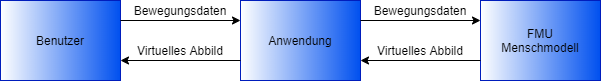
\includegraphics[width=1\linewidth]{Bilder/A23_FMUCoSimulation}
	\caption{Die beispielhafte Funktionsweise der FMU als Teil einer Anwendung, eigene Abbildung}
	\label{fig:FMUCoSimulation}
\end{figure}
\paragraph{ModelVariables}\label{sec:ModelVariables}
\noindent In dem Bereich “ModelVariables“ sind die Variablen der FMU definiert. Diese Variablen werden unter dem übergeordneten Typ „ScalarVariable“ gespeichert und erhalten alle einen eindeutigen Index. Des Weiteren sind „Scalar Variables“ primitive Variablen, wie z.B. ganze Zahlen (Integer), Texte (String) oder Wahrheitswerte (Boolean) (Vgl. Abbildung \ref{fig:FMIOverview}). Zusätzlich zu dem Variablentyp und Inhalt sind noch die optionalen Annotationen (Vgl. Abbildung \ref{fig:FMIOverview}) und die Attribute Bestandteil dieser Variablen \cite[S.45]{25}. 
\newline
Folgende Einträge gehören zu den \textbf{Attributen} der ModelVariables:
\begin{enumerate}
	\item \textbf{„name"} \cite[S.46]{25} \\
	Jede Variable erhält einen einzigartigen Namen und kann somit von der Instanz der FMU
	entweder über den Namen oder über Ihren Index aus der Liste aller ScalarVariables
	identifiziert werden \cite[S.46]{25}.
	\item \textbf{„valueReference" (Nur für C-Code)} \cite[S.46f]{25} \\
	Dieser Eintrag ermöglicht die eindeutige Zuordnung einer Variable durch die C-Functionen
	des Codes \cite[S.46f]{25}.
	\item \textbf{„description" (optional)} \cite[S.47]{25} \\
	Bei Bedarf kann jede Variable eine kurze Beschreibung enthalten, die das spätere Arbeiten
	mit der Variable erleichtern kann \cite[S.47]{25}.
	\item \textbf{„causality"} \cite[S.47]{25} \\
	Die Variablen können von unterschiedlicher Kausalität sein. Folgende Optionen stehen zur
	Verfügung \cite[S.47]{25}:
	\begin{enumerate}
		\item \textbf{„parameter"} \cite[S.47]{25} \\
		Falls es sich um eine Konstante handelt \cite[S.47]{25}.
		\item \textbf{„calculatedParameter"} \cite[S.47]{25} \\
		Falls es sich um Konstante handelt, die während jeder 
		Initialisierung der FMU neu berechnet werden muss \cite[S.47]{25}.
		\item \textbf{„input"} \cite[S.47]{25} \\
		Falls es sich um eine Eingabevariable handelt \cite[S.47]{25}.
		\item \textbf{„output"} \cite[S.47]{25} \\
		Falls es sich um eine Ausgabevariable handelt \cite[S.47]{25}.
		\item \textbf{„local"} \cite[S.47]{25} \\
		Falls die Variable ausschließlich von der FMU verwendet werden darf \cite[S.47]{25}.
		\item \textbf{„independent"} \cite[S.47]{25} \\
		Falls es sich um eine unabhängige Variable, wie z.B. Zeit handelt \cite[S.47]{25}.
	\end{enumerate}
	Die Standardeinstellungen für Variablen ist local \cite[S.47]{25}.
	\item \textbf{„variability"} \cite[S.48]{25} \\
	Durch diesen Eintrag kann definiert werden, inwiefern eine Variabel Zeitabhängig ist. Dabei
	stehende Optionen zur Verfügung \cite[S.48]{25}:
	\begin{enumerate}
		\item \textbf{„constant"} \cite[S.48]{25} \\
		Für Variablen die sich nicht über die Zeit verändern \cite[S.48]{25}.
		\item \textbf{„fixed"} \cite[S.48]{25} \\
		Für Variablen die sich nach Abschluss der Initialisierung nicht mehr verändern
		\cite[S.48]{25}.
		\item \textbf{„tunable"} \cite[S.48]{25} \\
		Für Variablen die zwischen Events (beim ModelExchange) und
		Kommunikationszeitpunkten (Co-Simulation) konstant sind \cite[S.48]{25}.
		\newpage
		\item \textbf{„discrete"} \cite[S.48]{25} \\
		Für Variablen die sich nicht durch Events (beim ModelExchange)
		verändern und nur zu bestimmten Kommunikationszeitpunkten (Co-Simulation) veränderbar
		sind \cite[S.48]{25}.
		\item \textbf{„continuous"} \cite[S.48]{25} \\
		Für Variablen die keine Restriktionen für Veränderungen haben \cite[S.48]{25}.
	\end{enumerate}
	Die Standardeinstellungen für Variablen ist continuous \cite[S.48]{25}.
	\item \textbf{„initial" (optional)} \cite[S.48f]{25} \\
	Dieser Eintrag beschreibt wie die Variable nach der Initialisierung aussieht. Dabei stehen
	folgende Optionen zur Verfügung \cite[S.48f]{25}:
	\begin{enumerate}
		\item \textbf{„exact"} \cite[S.48f]{25} \\
		Falls die Variable mit einem festen Startwert initialisiert wird \cite[S.48f]{25}.
		\item \textbf{„approx"} \cite[S.48f]{25} \\
		Falls die Variable mit einem approximierten Startwert initialisiert wird
		\cite[S.48f]{25}.
		\item \textbf{„calculated"} \cite[S.48f]{25} \\
		Falls die Variable mit einem aus anderen Variablen berechneten
		Startwert initialisiert wird \cite[S.48f]{25}.
	\end{enumerate}
	\item \textbf{„canHandleMultipleSetPerTimeInstant" (optional)} \cite[S.49]{25} \\
	Bei diesem Attribut gilt die Besonderheit, dass es nur beim Modellaustausch zum Einsatz
	kommt und daher bei der Co-Simulation vernachlässigt werden kann. Dieses Attribut soll 
	Informationen darüber liefern, ob eine Variable innerhalb desselben Zeitintervalls mehr als 
	einmal evaluiert werden kann und kann deshalb nur die Werte true (wahr) oder false (falsch) 
	annehmen \cite[S.49]{25}.
\end{enumerate}
In Abbildung \ref{fig:ModelVariables} wird anhand von einem Beispiel gezeigt, wie die ModelVariables auszusehen hätten. Dargestellt wird die Variable mit dem Namen „leftFootID“, welche die ID des Trackers für den linken Fuß als String abspeichert. Bei dieser Variable handelt es sich um einen konstanten Parameter, der mit dem exakten Startwert „LHR-C4F9A61E“ initialisiert wird. Es gibt keine weiteren optionalen Annotationen die zu dieser Variable gehören.
\begin{figure}[h]
	\centering
	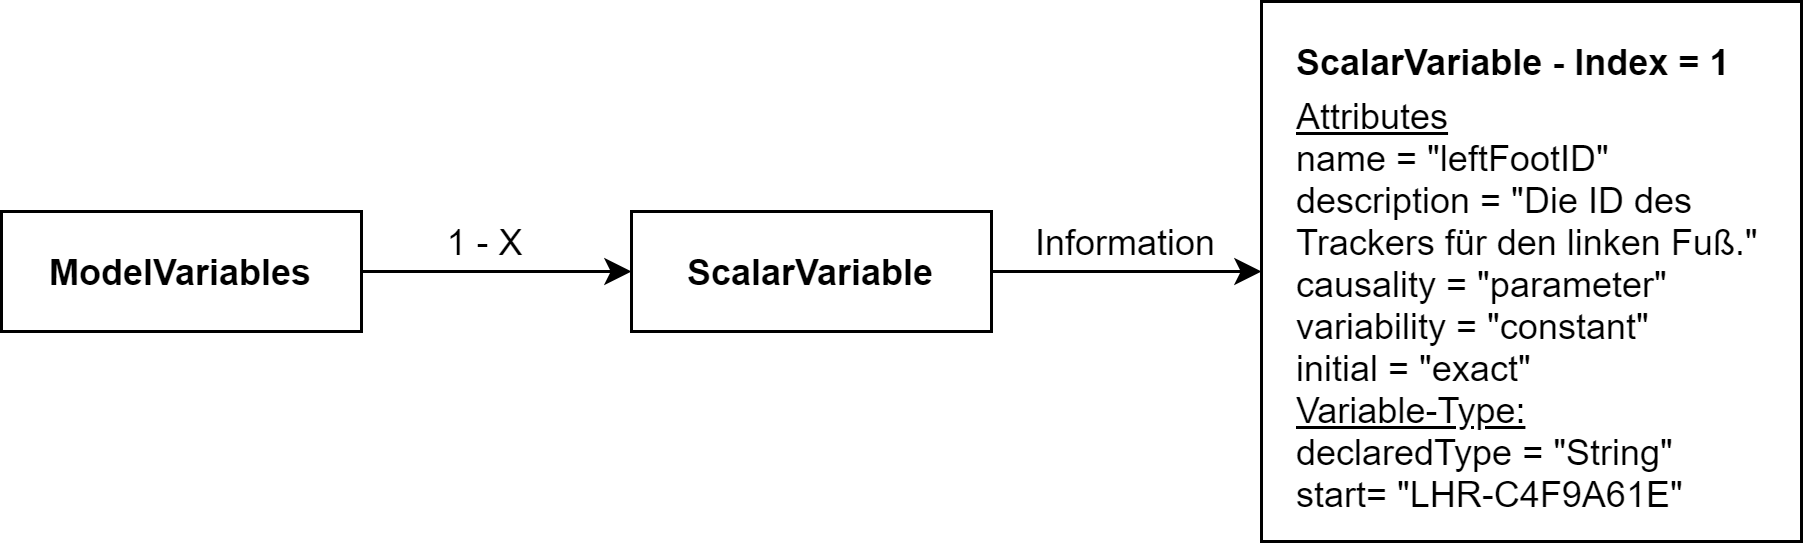
\includegraphics[width=1\linewidth]{Bilder/A30_ModelVariables}
	\caption{Die beispielhafte Darstellung des Aufbaus einer ModelVariable, eigene Abbildung}
	\label{fig:ModelVariables}
\end{figure}
\newpage
\paragraph{ModelStructure}\label{sec:ModelStructure}
\noindent In dem Bereich ModelStructure wird, wie der Name bereits vermuten lässt, die Modellstruktur definiert. Dabei werden die Outputs (Ausgabevariablen), Derivatives (Ableitungen) und InitialUnknowns (Anfänglich unbekannte Variablen) in geordneter Reihenfolge angegeben, sodass alle Tools dieselbe Reihenfolge für die Paramater verwenden \cite[S.57]{25}.
\begin{enumerate}
	\item \textbf{„Outputs"} \cite[S.60]{25} \\
	Enthält in einer geordneten Liste alle Ausgabevariablen der FMU. Alle Variablen mit der 
	Kausalität „output“ müssen in dieser Liste vorkommen \cite[S.60]{25}.
	\item \textbf{„Derivatives"} \cite[S.60f]{25} \\
	Enthält in einer geordneten Liste alle Ableitungen der FMU \cite[S.60f]{25}.
	\item \textbf{„InitialUknknows"} \cite[S.61]{25} \\
	Enthält in einer geordneten Liste alle Variablen, die zum Zeitpunkt der Initialisierung der FMU	noch unbekannte Werte besitzen. Alle Variablen mit der Kausalität „output“ in Kombination mit der Markierung „approx“ oder „calculated“ beim Startwert  und alle Variablen mit der Kausalität „calulatedParamter“ müssen in dieser Liste vorkommen \cite[S.61]{25}.
\end{enumerate}
Die einzelnen Elemente in den drei oben genannten Listen werden unter der übergeordneten Kategorie Unknown gespeichert (Vgl. Abbildung \ref{fig:FMIOverview}) und mit Hilfe des Index der entsprechenden ScalarVariable angegeben \cite[S.61]{25}. Insgesamt besitzen die Elemente folgende Attribute:
\begin{enumerate}
	\item \textbf{„index"} \cite[S.62]{25} \\
	Der Index gibt an auf welche Variable aus den zuvor definierten ModelVariables sich das 
	Element bezieht \cite[S.62]{25}.
	\item \textbf{„dependencies" (optional)} \cite[S.62]{25} \\
	Durch dieses Element werden Abhängigkeiten zwischen Variablen dargestellt. Eine Variable
	kann von einer oder sogar mehreren anderen Variablen abhängig sein \cite[S.62]{25}.
	\item \textbf{„dependenciesKind" (optional)} \cite[S.63]{25} \\
	Dieses Element ermöglicht es zusätzlich Angaben über die Variabilität der dependencies zu 
	machen \cite[S.63]{25}.
\end{enumerate}
So bedeutet beispielsweise <Uknown index  = “1“ dependencies = “2 3 4 5“ dependenciesKind=“constant constant fixed fixed”/>, dass die Variable mit dem Index 1 von den Variablen mit den Indizes 2, 3, 4 und 5 abhängig ist. Des Weiteren wird durch „dependenciesKind“ angegeben, dass die Variablen mit den Indizes 2 und 3 Konstanten sind, die sich nicht verändern und dass die Variablen mit den Indizes 4 und 5 sich nach dem Zeitpunkt der Initialisierung der FMU nicht mehr verändern.
\newline\newline
Im Folgenden wird in der Abbildung \ref{fig:ModelStructure}, Anhand von einer Teilmenge der Variablen der FMU, dargestellt, wie die ModelStructure auszusehen hätte. Es ist anzumerken, dass die Variablen mit den Indizes 1-7 alle vom Typ Integer sind und dafür da sind, um den Körperteilen den Index des zugehörigen Trackers zuzuweisen. Die Variablen mit den Indizes 8-14 sind alle vom Typ String und repräsentieren die eindeutige ID der einzelnen Tracker. Des Weiteren wird in der Abbildung \ref{fig:ModelStructure}, repräsentativ für die Variablen mit den Indizes 1-7 und 8-14, Anhand der Variablen mit den Indizes 1 und 8, ein Beispiel über den Aufbau der Variablen gegeben. Die Variablen mit den Indizes 1-7 sind veränderliche Output-Variablen vom Typ Integer ohne Startwert (Vgl. Abbildung \ref{fig:ModelStructure}) und die Variablen mit den Indizes 8-14 sind konstante Parameter mit einem exakten Startwert in Form eines Strings (Vgl. Abbildung \ref{fig:ModelStructure}). Die dargestellte Struktur besser zu verstehen, erfordert zu wissen zu wissen, dass die genutzte VR Brille die Tracker über einen eindeutigen Index identifiziert. Dabei bekommt jeder Tracker bei jeder erneuten Verbindung mit dem PC einen zufälligen Index zugewiesen. Bei der Zuweisung der Tracker wird, in Abhängigkeit der ID der einzelnen Tracker, den Körperteilen der entsprechende Index des dazugehörigen Trackers zugewiesen.
\begin{figure}[h]
	\centering
	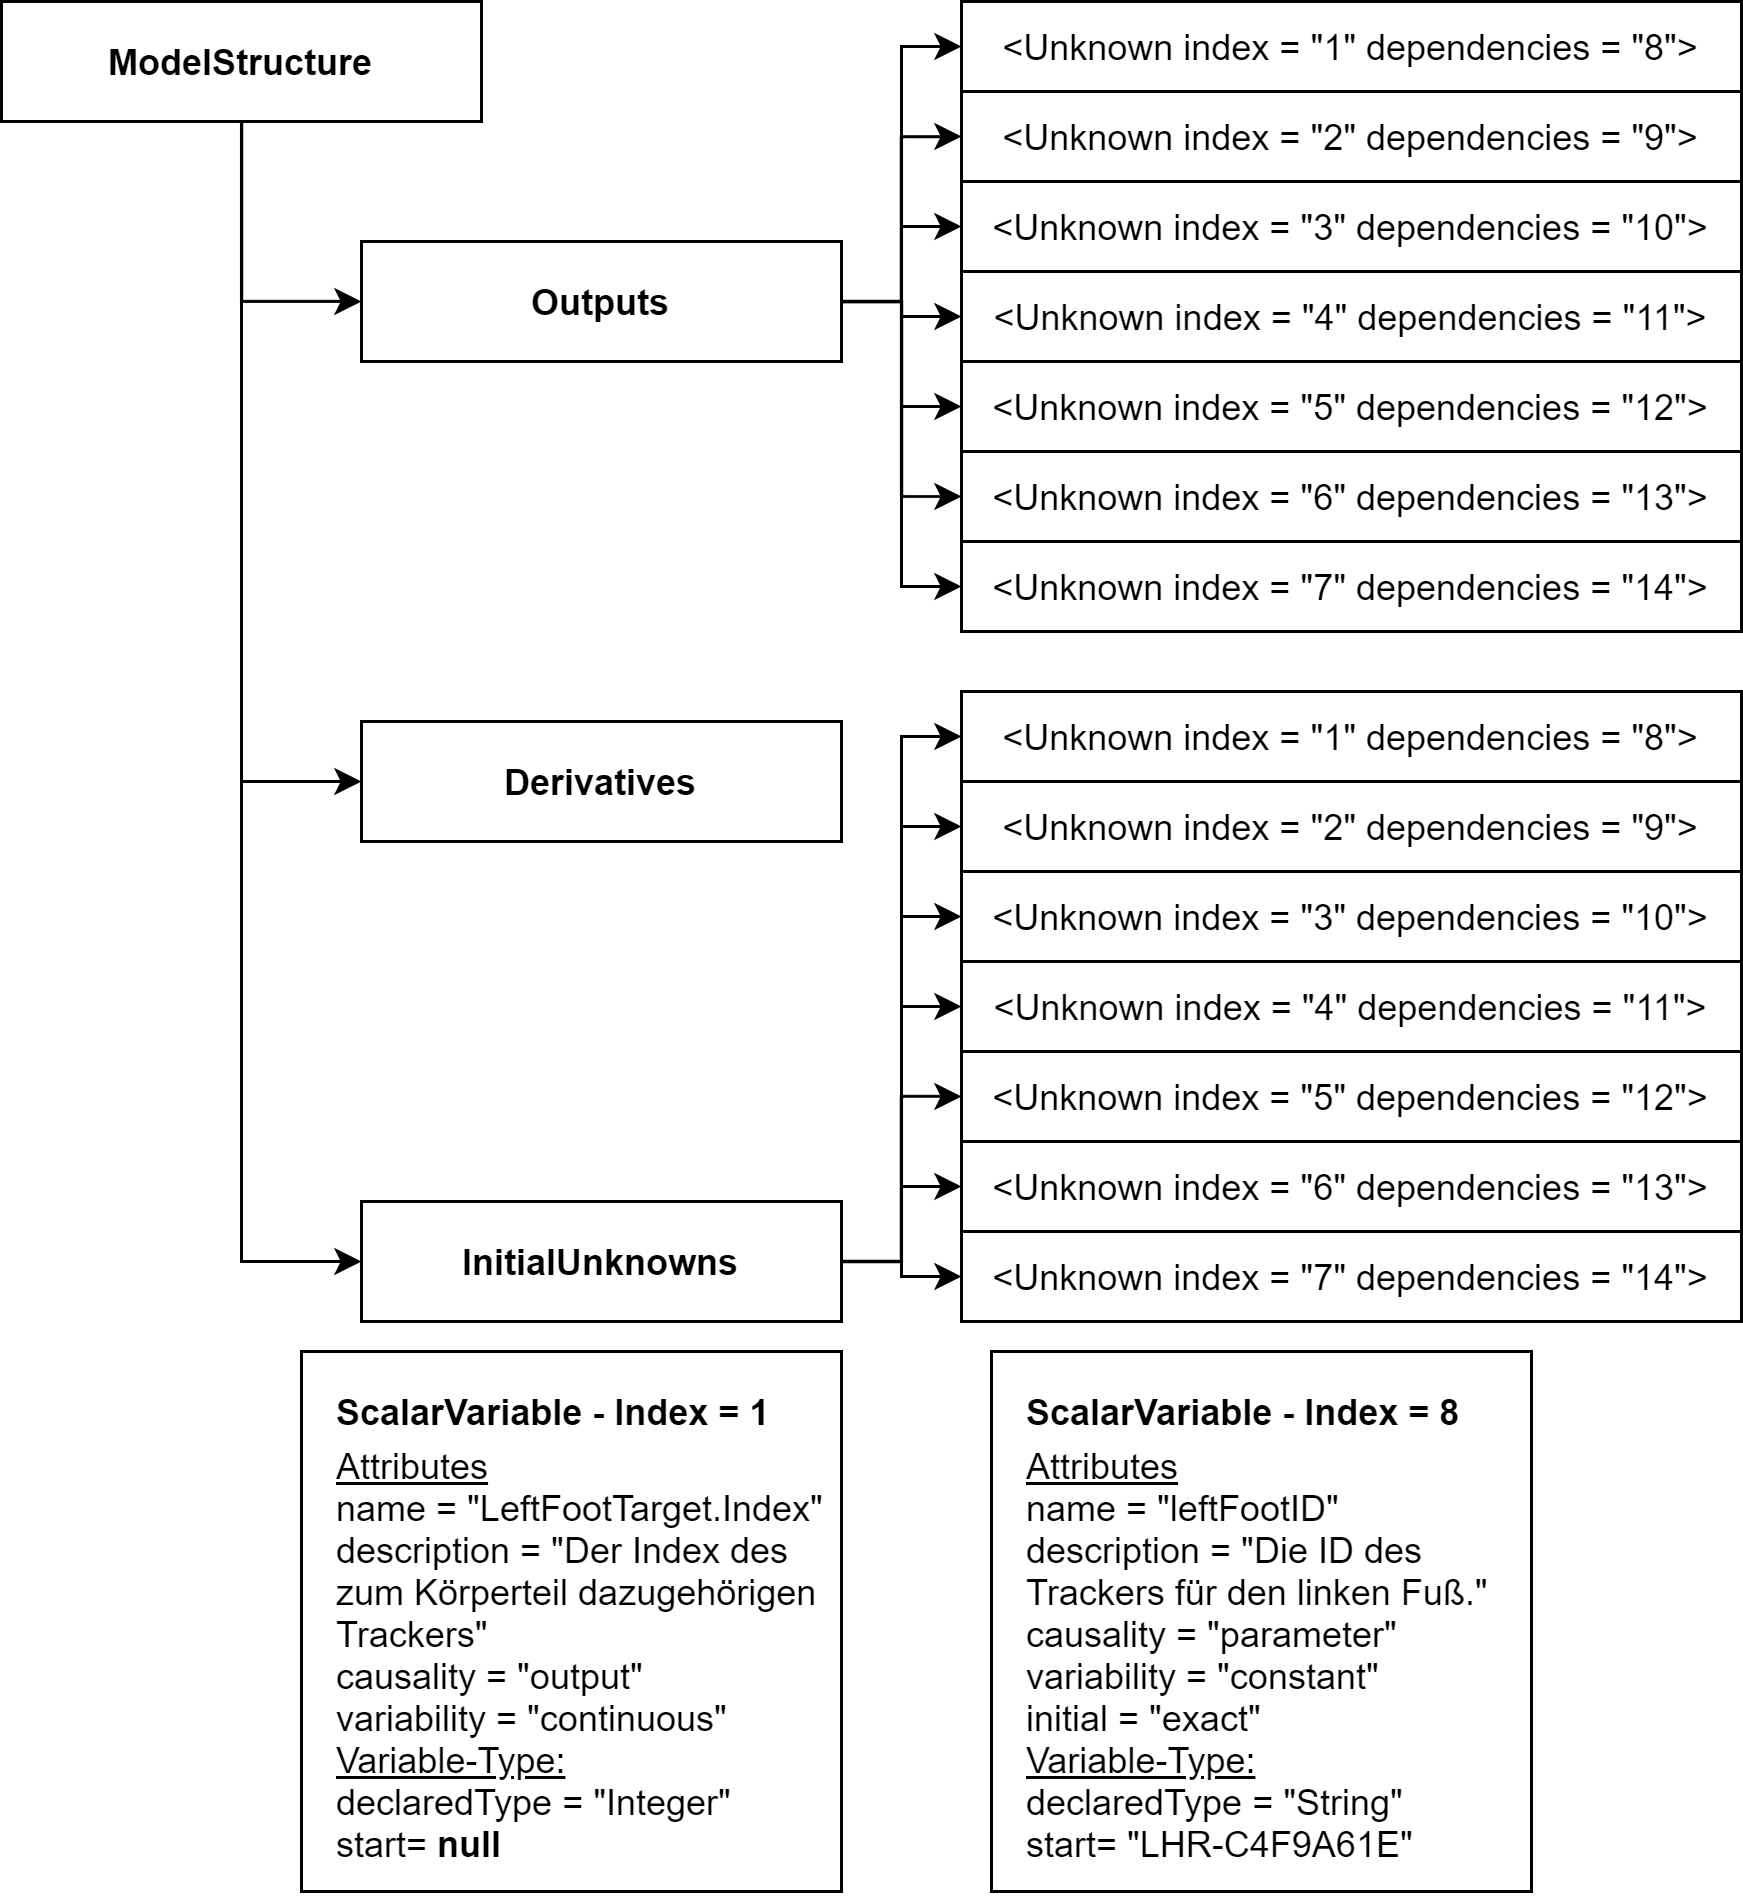
\includegraphics[width=0.85\linewidth]{Bilder/A31_ModelStructure}
	\caption{Die beispielhafte Darstellung der ModelStructure, eigene Abbildung}
	\label{fig:ModelStructure}
\end{figure}
\newpage
\paragraph{UnitDefinitions (optional)}\label{sec:UnitDefinitions}
\noindent Der Bereich UnitDefinitions ist optional und erlaubt den Entwicklern eigene Einheiten zu definieren.  Die einzelnen Elemente in diesem Bereich werden unter der übergeordneten Kategorie Unit gespeichert (Vgl. Abbildung \ref{fig:FMIOverview}). Eine Unit besteht aus den Komponenten Attributes, BaseUnit und DisplayUnit. Es ist anzumerken, dass eine Unit insgesamt nur ein Attribut (name) besitzt, welches dafür da ist um die Unit durch ihren Namen eindeutig identifizieren zu können \cite[S.34]{25}. Die Komponenten BaseUnit und Display Unit setzen sich wie folgt zusammen:
\begin{enumerate}
	\item \textbf{„BaseUnit"} \cite[S.35]{25} \\
	Durch die Komponente BaseUnit werden Einheiten definiert, um die Konvertierung zwischen
	verschiedenen Einheiten zu ermöglichen. Die BaseUnit Komponente besteht lediglich aus 
	Ihren eigenen Attributen, welche die verschiedenen Einheiten darstellen. Insgesamt sind 
	bereits zehn Einheiten standardmäßig vorhanden, dazu gehören Beispielweise die Einheiten 
	kg oder m \cite[S.35]{25}.
	\item \textbf{„DisplayUnit"} \cite[S.38]{25} \\
	Durch die Komponente DisplayUnit werden Einheiten in das gewünschte Input/Output
	Format konvertiert. Eine DisplayUnit besteht immer aus Ihren Attributen name (Name), 
	factor (Faktor) und offset (Abweichung). Dabei ist anzumerken, dass der Name eindeutig sein 
	muss. Die Umrechnung erfolgt stehts nach der Formel: Neuer Wert = Faktor * Wert + 
	Abweichung \cite[S.38]{25}.
\end{enumerate}
Für diese Arbeit würden keine UnitDefinitions zum Einsatz kommen.
\paragraph{TypeDefinitions (optional)}\label{sec:TypeDefinitions}
\noindent Der Bereich TypeDefinitions ist optional und erlaubt den Entwicklern eigene Zusammengesetze Typen zu erstellen. Die einzelnen Elemente in diesem Bereich werden unter der übergeordneten Kategorie SimpleType gespeichert (Vgl. Abbildung \ref{fig:FMIOverview}). Ein SimpleType besteht aus den Komponenten Attributes und den entsprechenden Variabletypen. Zu den Attributen einer SimpleType gehören nur die optionale Beschreibung (description) und ein eindeutiger Name (name). Zu den möglichen Variabletypen gehören unter anderem Integer (ganze Zahlen), Boolean (Wahrheitswerte) und Strings (Text) \cite[S.39]{25}.
\newline
Für diese Arbeit würden keine TypeDefinitions zum Einsatz kommen.
\paragraph{LogCategories (optional)}\label{sec:LogCategories}
\noindent Der Bereich LogCategories ist optional und erlaubt den Entwicklern den Output im Log (Konsole) in verschiedene Kategorien einzuordnen. Die einzelnen Elemente in diesem Bereich werden unter der übergeordneten Kategorie Category gespeichert (Vgl. Abbildung \ref{fig:FMIOverview}). Eine Category besteht aus den Attributen name (Name) und description (Beschreibung) \cite[S.43]{25}.
\newline
Für diese Arbeit würden keine LogCategories zum Einsatz kommen.
\paragraph{DefaultExperiment (optional)}\label{sec:DefaultExperiment}
\noindent Der Bereich DefaultExperiment ist optional und erlaubt den Entwicklern durch Startwerte eine Standardkonfiguration zu definieren. Insgesamt besteht der Bereich Default Experiment nur aus der Unterkategorie Attributes. Zu den Attributen gehören startTime (Start Zeit), stopTime (Stop Zeit), tolerance (Tolleranz) und stepSize (Schritt Größe) \cite[S.44]{25}.
\newline
Für diese Arbeit würde kein DefaultExperiment zum Einsatz kommen.
\paragraph{VendorAnnotations (optional)}\label{sec:VendorAnnotations}
\noindent Der Bereich VendorAnnotations ist optional und erlaubt den Entwicklern der FMU zusätzliche, toolspezifische Annotationen bzw. Informationen bereit zu stellen. Die einzelnen Elemente in diesem Bereich werden unter der übergeordneten Kategorie Tool gespeichert (Vgl. Abbildung \ref{fig:FMIOverview}). Ein Tool besteht aus dem Attribut name (Name) und den eigentlichen Informationen. Diese Informationen können in einem beliebigen XML-Format vorliegen \cite[S.45]{25}.
\newline
Für diese Arbeit würden keine VendorAnnotations zum Einsatz kommen.

\subsection{Die Potenziale des Functional-Mockup Interfaces}\label{sec:PotenzialeFMU}
Der FMI Standard bietet den Vorteil, dass durch die Unabhängigkeit von der genutzten Simulationsumgebung und die Standardisierung der Input- und Output-Schnittstellen, viele Module einfach zu einem großen Projekt zusammengefasst werden können. Dadurch können Module erweitert oder sogar ganz ausgetauscht werden.
Unter der Berücksichtigung der in Kapitel \ref{sec:AnforderungenKonzept} erläuterten Anforderungen Modularität und Interoperabilität und der in Kapitel \ref{sec:MMInteraktion} erläuterten zusammengesetzten Mensch-Maschine-Schnittstelle, würde die Einhaltung des FMI Standards ermöglichen, das Menschmodell mit geringen Aufwand mit einer geeigneten Infrastruktur für die Kommunikation zwischen dem Computer und Produktionsanlagen zu verbinden.
\newline
Somit ist steckt das größte Potential des FMI Standards in der Einhaltung der Modularität und Interoperabilität. Dies wird durch die freie Wahl der Simulationsumgebung und die Möglichkeit Co-Simulation einzusetzen weiterhin verstärkt, da die eingesetzten Module frei nach eigenen Wünschen implementiert und unabhängig von dem restlichen System eingesetzt werden können. Außerdem ist davon auszugehen, dass der FMI Standard den Unternehmen durchaus das Potential bietet, sich an die in Kapitel \ref{sec:AutomatisierungspyramideUndIndustrie4.0} erläuterte Auflösung der herkömmlichen Automatisierungspyramide anzupassen und somit in Zukunft Cloud-basierte und standortunabhängige Produktionsprozesse zu ermöglichen.
\newline
Schließlich sei noch zu erwähnen, dass auch Siemens das Potential des FMI Standards und vor allem der Co-Simulation erkannt hat. Dadurch, dass die Produktion immer Modularer wird und somit von immer mehr Zulieferern abhängig ist, bedarf es einer Schnittstelle für Co-Simulation, da eine einzige Simulationsumgebung nicht mehr effizient umsetzbar ist. Ein Grund dafür ist z.B. die Tatsache, dass die meisten Simulationstools nur eine begrenzte Anzahl an Formaten unterstützen. Die durch die Co-Simulation gewonnene Flexibilität bietet den Besitzern von Produktionsanlagen die Möglichkeit, auf unerwartete Veränderungen oder sogar Ausfälle schneller reagieren zu können\cite[S.13]{27}. 

%--------------------------------------------------------------------------------------------------